\chapter{Introduzione}
\lstset{basicstyle=\small\ttfamily,keywordstyle=\color{black}\bfseries,commentstyle=\color{darkgray},stringstyle=\color{black},showstringspaces=true}

Questa tesi ha come obbiettivo lo studio e l'analisi delle tecniche di spam detection attualmente esistenti ed in particolare delle tecniche online. Nella prima parte le tecniche verranno classificate sulla base dei segnali che utilizzano. Successivamente verranno eseguiti dei test per valutare alcuni algoritmi di spam detection offline eseguiti durante la fase di crawling. Ed infine verrano presentati e discussi i risultati ottenuti. Al momento in cui si scrive non ci sono, o meglio sono poche, le tecniche online di spam detection, ovvero tecniche che rilevano lo spam durante la fase di crawling. Infatti quasi tutti i metodi tentano di fare il crawling dell'intera porzione di web di interesse e successivamente classificare le pagine in classi (dove di norma le classi sono due: \textit{spam} oppure \textit{non spam}).

Il fenomeno del web spam è sempre più presente all'interno del web: questo è dovuto al fatto che gli utenti tendono ad esaminare solo i primi risultati calcolati dai motori di ricerca e quindi se un sito fa parte degli \textit{n} primi risultati può avere un ritorno economico legato alla quantità di traffico che viene generata per quel sito. Uno studio  del 2005 descritto in \cite{Nicholas:2005} stima che la perdita finanziaria mondiale causata dallo spam e di circa 50 miliardi di dollari e nel 2009 (come descritto in \cite{Nicholas:2009}) è salita a 130 miliardi di dollari. Per questo motivo, recentemente tutte le più grandi compagnie di motori di ricerca hanno identificato il recupero di informazioni non pertinenti come una delle priorità da risolvere. Le conseguenze del web spam possono essere riassunte come segue\cite{Spirin:2012:SWS:2207243.2207252}:
\begin{itemize}
 \item la qualità delle ricerche è compromessa penalizzando i siti web legittimi;
 \item un utente potrebbe perdere la fiducia sulla qualità di un motore di ricerca e perciò passare con facilità all'utilizzo di un altro;
 \item inoltre i siti spam possono essere usati come mezzo per malware, pubblicazione di contenuto per adulti e attacchi di tipo ``fishing''. Una prova tangibile si può vedere in \cite{Eiron:2004:RWF:988672.988714}, dove gli autori hanno eseguito l'algoritmo di \textit{PageRank} su 100 milioni di pagine e hanno notato che 11 sui primi 20 risultati erano composti da siti con contenuto per adulti.
\end{itemize}
Queste considerazioni evidenziano che quando si progetta un motore di ricerca bisogna tenere conto delle pagine che potrebbero portare al mal funzionamento del motore stesso.
%questa parte forse è da cambiare in quanto il lavoro sta cambiando infatti dallo sviluppo di un modulo siamo passati a fare dei test degli algoritmi di spam
%detection su grafo
Il lavoro prodotto sarà utilizzato per essere integrato	all'interno di un web crawler distribuito ad alte prestazioni per il futuro sviluppo di un modulo di spam detection. L'esigenza di tale modulo è sorta a seguito dello sviluppo, presso il Dipartimento, di un crawler chiamato {\itshape BUbiNG}, altamente configurabile ma privo al momento di qualunque forma di rilevazione di siti e contenuti malevoli. Il problema è estremamente interessante sia dal punto di vista teorico che da quello pratico: infatti, sebbene siano numerose le tecniche descritte in letteratura per la determinazione di spam (usando come segnali sia il contenuto che la struttura dei link), è sorprendentemente scarso l'insieme di tali tecniche che possono essere usate on-line, cioè durante il crawl. Il problema diventa ancora più complesso se si aggiungono considerazioni legate ai vincoli di spazio di memoria disponibile e tempo di calcolo.
Infatti in letteratura il processo di spam detection viene eseguito subito dopo la fase di crawling. Ovvero il processo è composto dai seguenti passi:
\begin{itemize}
 \item crawling dell'intero web;
 \item fase di spam detection;
 \item indicizzazione.
\end{itemize}
Questo modello è utile perché molte delle tecniche utilizzate fanno delle analisi sul grafo che è il risultato della fine del processo di crawling. Da queste considerazioni noi proviamo a fare delle analisi per determinare se il processo di spam detection può essere fatto durante la fase di crawling ovvero al momento in cui il crawler esegue il ``fetch'' di una pagina per determinare ``on the fly'' se la pagina è buona o ha un contenuto malevolo. 

\section{Ranking dei motori di ricerca}
Prima di spiegare i vari metodi con cui si possono creare pagine web spam e successivamente quelli utili ad identificarlo, è necessario capire come i motori di ricerca sono capaci di valutare la rilevanza di una pagina web per una determinata query.
%preso dalle dispense

In linea di massima un sistema di reperimento di informazioni ovvero un motore di ricerca è dato da una collezione documentale \textit{D} (un insieme di documenti) di dimensione \textit{N} , da un insieme \textit{Q} di interrogazioni, e da funzione di ranking (\(r : Q \times D \rightarrow R\)) che
assegna a ogni coppia formata da un’interrogazione e un documento un numero reale. L’idea è che a fronte di un’interrogazione a ogni documento viene assegnato un punteggio reale: i documenti con punteggio nullo non sono considerati rilevanti, mentre quelli a punteggio non nullo sono tanto più rilevanti quanto più il punteggio è alto. In particolare i metodi di ranking si dividono in \textit{endogeni} ed \textit{esogeni}. I primi metodi fanno uso del contenuto del documento per valutarne la rilevanza mentre i secondi fanno uso di un struttura esterna ad esempio il grafo composto dai collegamenti ipertestuali tra le pagine web, questo non implica che i metodi esogeni non possono fare uso del contenuto della pagina (per esempio il testo delle ancore). I criteri si dividono ulteriormente in statici (o indipendenti dall’interrogazione) e dinamici (o dipendenti dall’interrogazione). Nel primo caso, il punteggio assegnato a ciascun documento è fisso e indipendente da un'interrogazione \textit{q} mentre nel secondo il punteggio assegnato a ciascun documento e dipendente da un'interrogazione \textit{q}.

Tra i metodi endogeni sono di maggiore importanza \textit{tf-idf} e \textit{BM25} mentre tra quelli esogeni i più diffusi in letteratura sono \textit{PageRank} e \textit{HITS}.

\subsection{Metodi di ranking endogeno}
Come già detto i precedenza i metodi di ranking endogeno utilizzano il contenuto di una pagina per assegnarle un punteggio. Possono essere anch’essi statici o dinamici (cioè dipendere o meno da un’interrogazione). L'algoritmo usato dai motori di ricerca per fare il rank delle pagine web basandosi sui campi di testo usa varie forme del \textit{tf-idf}. Il \textit{tf-idf} e un metodo di ranking endogeno dinamico che utilizza il contenuto di una pagina per assegnarle un punteggio. Il \textit{tf-idf} è una misura composta da due misure più semplici: la \textit{Term Frequency} e la \textit{Inverse Document Frequency}. Il primo metodo assegna a un documento \textit{d} il punteggio dato dalla somma dei conteggi dei termini \textit{t} dell'interrogazione che compaiono nel documento stesso. In questo modo documenti in cui i termini dell'interrogazione compaiono più frequentemente avranno un punteggio più elevato. Utilizzare solo questo metodo non conviene in quanto è facilmente manipolabile. Inoltre non tiene conto del fatto che alcuni termini occorrono più frequentemente non perché rilevanti, ma perché altamente frequenti all'interno di \textit{ogni} documento (ad esempio le congiunzioni). Il secondo metodo è definito come l'inverso del numero di documenti nella collezione che contengono il termine \textit{t} \cite{Manning:2008:IIR:1394399p117}. Più precisamente:
\begin{equation}
 idf_t=\log\frac{N}{df_t}
 \label{eq:idf}
\end{equation}
La combinazione del \textit{tf} ed dell'\textit{idf} produce una misura composta che permette di normalizzare il peso dei termini. Il \textit{tf-idf} di un documento \textit{d} rispetto a una query \textit{q} è calcolato su tutti i termini \textit{t} in comune come:
\begin{equation}
 tf-idf(d,q)=\sum_{t \in d \: and \: t \in q} tf(t,d) \cdot idf(t)
\end{equation}
Con il \textit{tf-idf} gli spammer possono avere due obbiettivi: o creare pagine rilevanti per un gran numero di query o creare pagine molto rilevanti per una specifica query. Il primo obbiettivo può essere ottenuto includendo un gran numero di termini distinti in un documento; il secondo, attraverso la ripetizione di determinati termini nel documento.

Un altro metodo di ranking endogeno dinamico è \textit{BM25} \cite{Robertson:2009:PRF:1704809.1704810} che è uno schema di pesatura basato sul \textit{modello probabilistico} ed attualmente è il sistema di pesatura più usato. 

\subsection{Metodi di ranking esogeno}
Uno dei metodi esogeni statici è \textit{PageRank} descritto in \cite{ilprints422}. PageRank usa le informazioni portate dai link in entrata (\textit{inlink}) per determinare un punteggio globale di importanza di una pagina. Esso assume che esista un legame tra il numero di \textit{inlink} di una pagina \textit{p} e la popolarità della pagina \textit{p}. Il concetto fondamentale dietro \textit{PageRank} è che una pagina è importante se molte altre pagine importanti puntano ad essa. Questo concetto è mutualmente rinforzante ovvero l'importanza di una certa pagina influenza ed è influenzata dall'importanza delle altre pagine \cite{ilprints646}. In dettaglio \textit{PageRank} è basato sulla passeggiata naturale del grafo del web \textit{G}. Più precisamente, la passeggiata viene perturbata nel seguente modo: fissato un parametro \(\alpha\) tra \(0\) e \(1\), a ogni passo con probabilità \(\alpha\) si segue un arco uscente, e con probabilità \(1- \alpha \) si sceglie un qualunque altro nodo del grafo utilizzando una 
qualche 
distribuzione \(v\), detta
vettore di preferenza (per esempio, uniforme). Assumendo che non esistano pozzi, la matrice di transizione della catena è quindi rappresentata dalla combinazione lineare:
\begin{equation}
 \alpha G + (1 - \alpha) 1 v^T
\end{equation}
dove \(G\) è la matrice della passeggiata naturale su \(G\). Il fattore \(\alpha\) è detto fattore di attenuazione di norma è impostato a un valore di 0,85.

Un altro metodo esogeno usato per il ranking delle pagine è \textit{HITS (Hyperlink Induced Topic Distillation)} introdotto in \cite{Kleinberg:1999:ASH:324133.324140}. Differentemente da \textit{PageRank} esso assegna due punteggi di importanza a ogni pagina: uno di \textit{hubbines} e uno di \textit{autorevolezza}. L’intuizione dietro a HITS è che invece di un singolo punteggio di importanza esista un concetto di pagina \textit{autorevole}, cioè pagina con contenuto pertinente e interessante, e di \textit{hub}, cioè pagina contenente numerosi collegamenti a pagine autorevoli. I due concetti si rinforzano \textit{mutuamente}: una pagina autorevole è puntata da molte pagine centrali, e una buona pagina centrale punta a molte pagine autorevoli.

Questo approccio considera che nel web ci sono due tipi di pagine: quelle che contengono dei contenuti per un determinato argomento (\textit{authoritative}) e quelle che contengono tanti link a delle pagine \textit{authoritative} che sono chiamate pagine \textit{hub}. Le pagine \textit{hub} sono utili per scoprire le pagine \textit{authoritative} \cite{Manning:2008:IIR:1394399p474}.

L'algoritmo lavora su un sottografo del web ottenuto a partire da un'interrogazione. La selezione del sottografo può essere fatta in vari modi, un modo è quello di prendere un certo insieme di risultati  ottenuto da un motore di base e generare un sottografo sulla base di una query e delle pagine che puntano a quelle ottenute dalla query. Per questo sottoinsieme di pagine otteniamo un matrice di adiacenza \(A\). I punteggi di \textit{hub} e \textit{authority} per tutte le pagine del sottoinsieme possono essere formalizzate dalla seguente coppia di equazioni:
\begin{equation}
 \left\{
 \begin{array}{cc}
    \stackrel{\rightarrow}{a_{t+1}} \: = \: A^T \stackrel{\rightarrow}{h_t}\\
    \stackrel{\rightarrow}{h_{t+1}} \:= A \: \stackrel{\rightarrow}{a_{t+1}}
 \end{array}
 \right .
 \label{eq:hubat}
\end{equation}
Può essere dimostrato che la soluzione ottenuta applicando iterativamente il sistema \ref{eq:hubat} converge rispettivamente al principale autovettore di \(AA^T\) e \(A^TA\) \cite{Manning:2008:IIR:1394399p474}\cite{Spirin:2012:SWS:2207243.2207252}.

\section{Web spam}
Con il termine web spamming si fa riferimento a tutti i metodi che tentano di manipolare gli algoritmi di ranking dei motori di ricerca per aumentare il valore di alcune pagine rispetto ad altre \cite{ilprints646}.
Dato il numero esorbitante di pagine che vengono create e pubblicate sul web, gli utenti competono per far comparire le proprie pagine tra le prime dei risultati di una query.
Il fenomeno dello spamming o spamindexing ricade sulla qualità delle ricerche causando diversi problemi: indicizzazione di pagine che non sono utili, aumento del costo delle operazioni di query, malware e reindirizzamento verso contenuto per adulti; inoltre questo spinge gli utenti ad utilizzare altri motori di ricerca \cite{Spirin:2012:SWS:2207243.2207252}.

L'obbiettivo del motori di ricerca è di ottenere ottimi risultati per identificare tutte le pagine web che sono rilevanti per una specifica query e presentarle secondo l'importanza che esse hanno. Di norma la rilevanza viene misurata attraverso la similarità testuale tra la query e le pagine mentre l'importanza è definita come la popolarità globale della pagina e a volte è inferita dalla struttura dei link \cite{ilprints646}. Ci sono due categorie di tecniche associate al web spam \cite{ilprints646}:
\begin{itemize}
\item \textbf{tecniche boost} che cercano di far avere più importanza o rilevanza a delle pagine
\item \textbf{tecniche hiding} che sono metodi per nascondere le tecniche di boost all'utente dal browser, anche se alcuni autori incorporano queste tecniche fra quelle di boost.
\end{itemize}

\subsection{Tecniche di boost}
Le tecniche di boosting si dividono in: \textit{Term Spamming} e \textit{Link Spamming}. Con l'avvento degli algoritmi di ranking basati sulla struttura del grafo il \textit{Term Spaming} è stato trascurato. In figura \ref{fig:tassonomiaTecnicheBoost} è specificata una possibile tassonomia delle tecniche boost \cite{ilprints646}.
\begin{figure} 
 \centering
 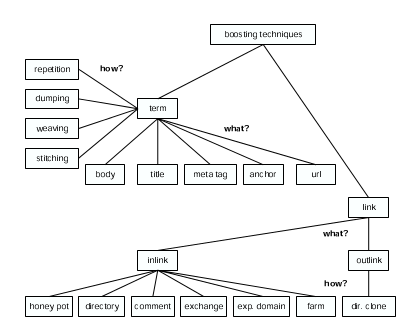
\includegraphics[width=10cm]{immagini/tassonomiaTecnicheBoost}
 \caption{Tassonomia delle tecniche boost}
 \label{fig:tassonomiaTecnicheBoost}
\end{figure}

\subsection{Term Spamming}
Nel valutare la rilevanza testuale i motori di ricerca considerano dove i termini di una query compaiono in una pagina. Il tipo di punto all'interno della pagina è chiamato \textit{campo}. I più comuni campi di testo per una pagina \textit{p} sono: il body della pagina, il titolo, i meta tag nell'header HTML e l'URL della pagina. Inoltre viene considerato anche come \textit{campo}, il testo delle ancore (il tag \textit{a}) associate all'URL che puntano alla pagina \textit{p} dato che descrive molto bene il contenuto della pagina . I campi di testo  di \textit{p} sono utilizzati per determinare la rilevanza di \textit{p} rispetto ad una query (alcune volte i campi vengono pesati sulla base della loro importanza) e perciò chi fa \textit{term spamming} utilizza tecniche di pesatura dei contenuti dei campi di testo in modo tale da aumentare l'efficacia dello spam \cite{ilprints646}. Le tecniche di spamming possono essere raggruppate in base ai \textit{campi} di testo dove viene fatto spamming. In base a 
questo distinguiamo \cite{ilprints646}:
\begin{itemize}
\item \textit{Body Spam}. In questo caso lo spam è nel corpo del documento. Questo è lo spam più diffuso.
\item \textit{Title Spam}. Molti motori di ricerca danno molta importanza ai termini che compaiono nel titolo. Quindi ha senso includere termini di spam all'interno del titolo della pagina.
\item \textit{Meta Tag Spam}. I tag che compaiono nell'header sono molto frequentemente soggetti a spam. Per questo i motori di ricerca danno poca importanza a questi campi o non li considerano. Di seguito viene mostrato un esempio di questo tipo di spam.
\begin{lstlisting}[frame=trbl,postbreak=\space, breakindent=5pt, breaklines]
 <meta name="keyword" content="buy, cheap, cameras, lens, accessories, nikon, canon">
\end{lstlisting}
\item \textit{Anchor Text Spam}. I motori di ricerca assegnano un peso maggiore al testo nelle ancore perché pensano che esse contengano un riassunto del contenuto della pagina. Perciò del testo di spam è incluso nel testo delle ancore dei collegamenti HTML di una pagina. In questo caso lo spamming non viene fatto sulla pagina cui si vuole far avere un rank più alto ma sulle pagine che puntano ad essa.
\begin{lstlisting}[frame=trbl,postbreak=\space, breakindent=5pt, breaklines]
<a href="target.html">free, great deals, cheap, inexpensive, cheap, free</a>
\end{lstlisting}
\item \textit{URL Spam}. Alcuni motori di ricerca dividono l'URL delle pagine in un insieme di termini che sono usati per determinare la rilevanza di una pagina. Per sfruttare questo metodo di ranking, gli spammer creano lunghi URL che includono una grande sequenza di termini spam, un esempio può essere: \textit{buy-canon-rebel-20d-lens-case.camerasx.com}.
\end{itemize}
Queste tecniche possono essere utilizzate insieme o separatamente. Un altro modo per raggruppare queste tecniche si basa sul tipo di termini che vengono utilizzati nei campi di testo \cite{ilprints646}, possiamo avere:
\begin{itemize}
\item Ripetizione di uno o più specifici termini.
\item Inclusione di molti termini generici per creare pagine rilevanti per molte query.
\item Intreccio di vari termini all'interno della pagina.
\item Creazione di frasi di senso compiuto per l'elaborazione di contenuti generati velocemente attraverso la concatenazione di frasi da fonti diverse.
\end{itemize}

\subsection{Link Spamming}
Il \textit{link spamming} è un tipo di spam che fa uso della struttura dei link tra le pagine web per favorire il rank di una pagina target \textit{t}.
In \cite{ilprints646} si afferma che per uno spammer ci sono tre tipi di pagine nel Web: inaccessibili, accessibili(blog) e proprietarie (fig. \ref{fig:tipologiaPagine}). Le inaccessibili sono quelle che uno spammer non può modificare. Le accessibili sono pagine gestite da altri ma che possono essere modificate lievemente dallo spammer attraverso l'immissione di un post in un forum o in un blog o portali di questo genere. Le proprietarie sono pagine su cui gli spammer hanno il pieno controllo. Il gruppo di pagine proprietarie è chiamato \textit{spam farm}.
\begin{figure} 
 \centering
 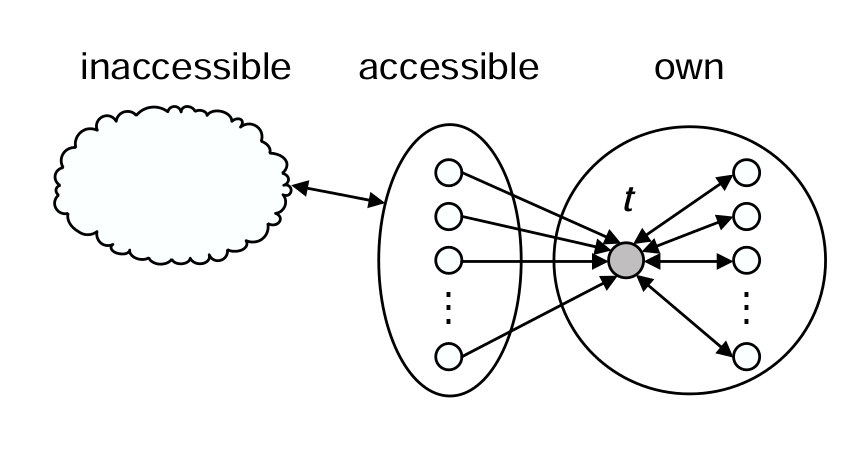
\includegraphics[width=10cm]{immagini/tipologiaPagine}
 \caption{Tipi di pagine nel web per uno spammer}
 \label{fig:tipologiaPagine}
\end{figure}

Molti motori di ricerca utilizzano due algoritmi per aumentare l'importanza basandosi sulle informazioni dei link: PageRank e HITS; sulla base di questi due tipi di algoritmi vengono definite due categorie principali di \textit{link spamming}: \textit{outgoing link spam} e \textit{incomign link spam}. L'\textit{outgoing link} è uno dei metodi più facili da implementare in quanto basta aggiungere dei link nella propria pagina, ad altre pagine che sono considerate buone, sperando di poter aumentare il  punteggio di \textit{hub}. Per la ricerca di link da includere nella pagina per cui si vuole incrementare il punteggio di \textit{hub} si possono utilizzare delle directory che contengono liste di siti come DMOZ o Yahoo!. Queste directory organizzano i contenuti web in contenuti e in liste di siti relativi. Per quanto riguarda \textit{incoming link}, ci sono diverse strategie che si possono adottare in modo tale da avere un numero elevato di link in entrata \cite{ilprints646}:
\begin{itemize}
\item \textit{Honeypot}: ovvero si creano un insieme di pagine che hanno un contenuto interessante (un esempio può essere una documentazione Linux) ma che hanno link nascosti alla pagina o alle pagine per cui si deve aumentare il valore di rilevanza.  
\item \textit{Infiltrarsi in una directory web}: molte directory web permettono ai webmasters di postare link ai loro siti che hanno lo stesso contenuto.
\item \textit{Postare link nei blog, forum e wiki}: includere URL a pagine di spam come parte di un commento.
\item \textit{Scambio di link}: scambiare link con altre pagine di spam. Questa è una pratica comune tra chi fa spam ed esistono blog completamente finalizzati all'incontro di spammer per lo scambio dei link.
\item \textit{Comprare domini scaduti}: quando un dominio scade ci sono delle pagine che puntano ancora ad esso. Una tecnica è comprare questi domini e manipolare le pagine in modo tale da fare aumentare il rank di una pagina target.
\item \textit{Creare una spam farm}: con l'abbassamento dei costi si possono costruire delle spam farm che hanno come obbiettivo di aumentare la rilevanza di un pagina spam detta \textit{target page}, un esempio è mostrato in fig. \ref{fig:spamfarm}. Molte volte si utilizzano tecniche come \textit{honeypot}. In questo caso il valore di page rank aggregato delle pagine è propagato alla pagina target. Una delle forme più aggressive di honeypot è l'\textit{hijacking} \cite{Spirin:2012:SWS:2207243.2207252}, dove gli spammer prima attaccano un sito con una buona reputabilità e poi usano questo come parte della loro link farm.
\end{itemize}
\begin{figure} 
 \centering
 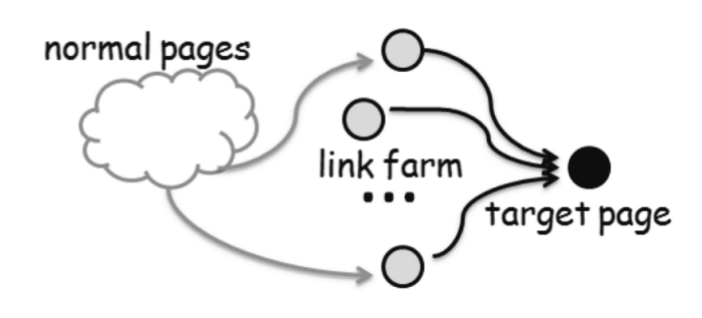
\includegraphics[width=10cm]{immagini/spamfarm}
 \caption{Esempio di una spamfarm}
 \label{fig:spamfarm}
\end{figure}

\subsection{Tecniche di hiding}
Le tecniche di hiding si possono classificare in: \textit{content hiding}, \textit{cloaking}, \textit{redirection} (fig. \ref{fig:tecnicheHiding}) \cite{ilprints646}.
\begin{figure} 
 \centering
 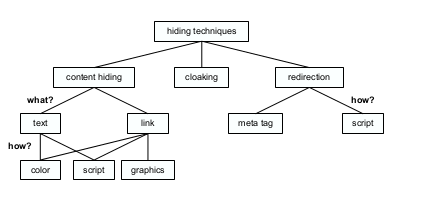
\includegraphics[width=10cm]{immagini/tassonomiaHiding}
 \caption{Tecniche di hiding}
 \label{fig:tecnicheHiding}
\end{figure}
Nel \textit{Content hiding} i termini o link di spam possono essere nascosti quando il browser visualizza una pagina. Una tecnica è quella di utilizzare lo stesso colore per i termini e lo sfondo. Mentre per i link basta non inserire il testo all'interno delle ancore che indirizzano a una pagina. Un'altra tecnica è quella di utilizzare degli script per nascondere il contenuto. Il \textit{Cloaking} sfrutta il fatto che è facile identificare quando la richiesta di una pagina è fatta da un crawler o da un browser: questa tecnica dato un URL, il server spam restituisce un documento HTML diverso a seconda che la richiesta sia fatta da un crawler o da un browser. Quindi vengono distribuiti due contenuti diversi in base al fatto che la richiesta al server spam sia fatta da un crawler o da un browser. La rilevazione di un crawler può essere effettuata in due modi: o si mantiene in memoria una lista di indirizzi di crawler oppure si usa l'header della richiesta HTTP andando a vedere il campo user-agent: se questo è diverso dai 
più comuni browser allora può essere un crawler. Nell'esempio sotto, lo user-agent della richiesta HTML indica l'uso del web browser Chrome.
\begin{lstlisting}[frame=trbl,postbreak=\space, breakindent=5pt, breaklines]
Mozilla/5.0 (X11; Linux x86_64) 
AppleWebKit/537.36 (KHTML, like Gecko) 
Chrome/32.0.1700.102 Safari/537.36
\end{lstlisting}
La \textit{Redirection} è un'altra tecnica che reindirizza il browser ad un altro URL appena la pagina è caricata. Un esempio di redirection server-side è mostrato di seguito.
\begin{lstlisting}[frame=trbl,postbreak=\space, breakindent=5pt, breaklines]
header("Location: http://www.example.com/");
\end{lstlisting}
\subsection{Click Spamming}
Un ultimo metodo per fare web spam è il \textit{Click Spamming} \cite{Spirin:2012:SWS:2207243.2207252}. I motori di ricerca utilizzano dati sul flusso dei click per regolare le funzioni di ranking, quindi  gli spammer generano clik fraudolenti per manipolare il comportamento di queste funzioni in modo tale da fare avere un rank migliore ai loro siti. Il metodo prevede che vengano fatte delle query e si clicchi sulla pagina di cui si vuole aumentare il rank. Tale metodo viene eseguito in modo automatico attraverso script che girano su diverse macchine per non fare sospettare il motore di ricerca delle numerose richieste provenienti da un unica macchina \cite{Spirin:2012:SWS:2207243.2207252}.


